\documentclass[10pt, a4paper]{article}
\usepackage{geometry}
\usepackage{graphicx}
\usepackage{amsmath}
\usepackage{hyperref}
\usepackage[english]{babel}
\usepackage{fancyhdr}
\usepackage[font=small, labelfont=bf]{caption}
\usepackage{biblatex}
\usepackage{microtype}
\usepackage{enumitem}
\usepackage{wrapfig}

\let\olditemize\itemize
\renewcommand{\itemize}{\olditemize[itemsep=0pt, parsep=0pt, topsep=0pt, partopsep=0pt]}
\let\oldenumerate\enumerate
\renewcommand{\enumerate}{\oldenumerate[itemsep=0pt, parsep=0pt, topsep=0pt, partopsep=0pt, leftmargin=9pt, labelwidth=0pt, labelsep=.5em]}

\addbibresource{references.bib}

\begin{document}

\begin{center}
{\Huge \textbf{Flooduino}}\\
\vspace*{1cm}
{\textbf{\LARGE University of Basel\\ \Large {Department for Mathematics and Informatics}}}\\
\vspace*{0.5cm}
{\Large Lecture Computer Architecture}\\
\vspace*{0.5cm}
Pascal von Fellenberg\\ Istref Uka\\ Frederic Weyssow\\ Alexander Marggraf\\
\vspace*{0.5cm}
\today
\end{center}

\section*{Abstract}

The goal of this project was to create our own implementation of the game Flood-it on an Arduino.  The outcome is a fully functioning implementation of the game encased in a cardboard housing which resembles an old arcade machine. To do this we used an Arduino Mega, a LED-matrix, a DFplayer Mini along with a speaker and three Buttons. Furthermore all of our own code is written in C and the project is compiled using the Arduino IDE. Everything is coordinated by the Arduino Mega on which the LED-matrix, a DFplayer Mini and the buttons are connected. The LED-matrix displays the current state of the game, the DFplayer Mini along with the speaker play music depending on the different stages and the three buttons allow the player to interact with the device. At the end of our project, everything worked as intended although not always on the first attempt. 

\section*{Introduction}

The goal of the game Flood-it is to fill a grid of differently colored cells with the same color in the maximal number of allowed moves. To start with the player can choose the size of the grid and how many colors should appear on the grid. Then each move the player can choose the color of the top left cell which is then propagated down the grid using a flood fill algorithm at the end of each move. If the player manages to use no more than some predetermined number of moves he wins, however if he uses more moves he loses.\\\\
To do this we used The Arduino Mega which was beneficial for us because of its increased memory capacity and its many connection pins. In addition we used a 64x64 LED-matrix from Waveshare as visual output, a DFplayer Mini to control the music, a Speaker for auditory output and three buttons as input. The LED-matrix always displays whatever stage the game is in at the current moment. These being the start screen, selection screen, the game and a win/loss screen. The DFplayer Mini functions similarly as it plays different music depending on the different stages of the game. The buttons consist of the arrow keys up and down as well as an enter key. The arrow keys are used to increase or decrease the field size and the amount of colors used in the selection screen and as a way to select the color in the game itself. The enter key is used every where else meaning to switch to the next stage and to initiate the flood fill algorithm.\\\\
We first created a prototype using C and raylib which is able to be run on any computer. Then we migrated this code over to the Arduino where changes were made wherever necessary. This includes using an Adafruit library instead of raylib for the visual output. Implementing controls for the DFplayer Mini as well as detecting the button presses. Next everything was build together using two breadboards, one for the buttons and one for the DFplayer Mini. Necessary connections between the devices where made using wires and transistors. Finally a cardboard housing was build which is made out of cardboard boxes that we bought in a hardware store. The shape was cut out and glued together using hot glue such that it resembles an old arcade.
\begin{figure}[h]
    \centering
    \begin{minipage}{0.48\linewidth}
    \centering
    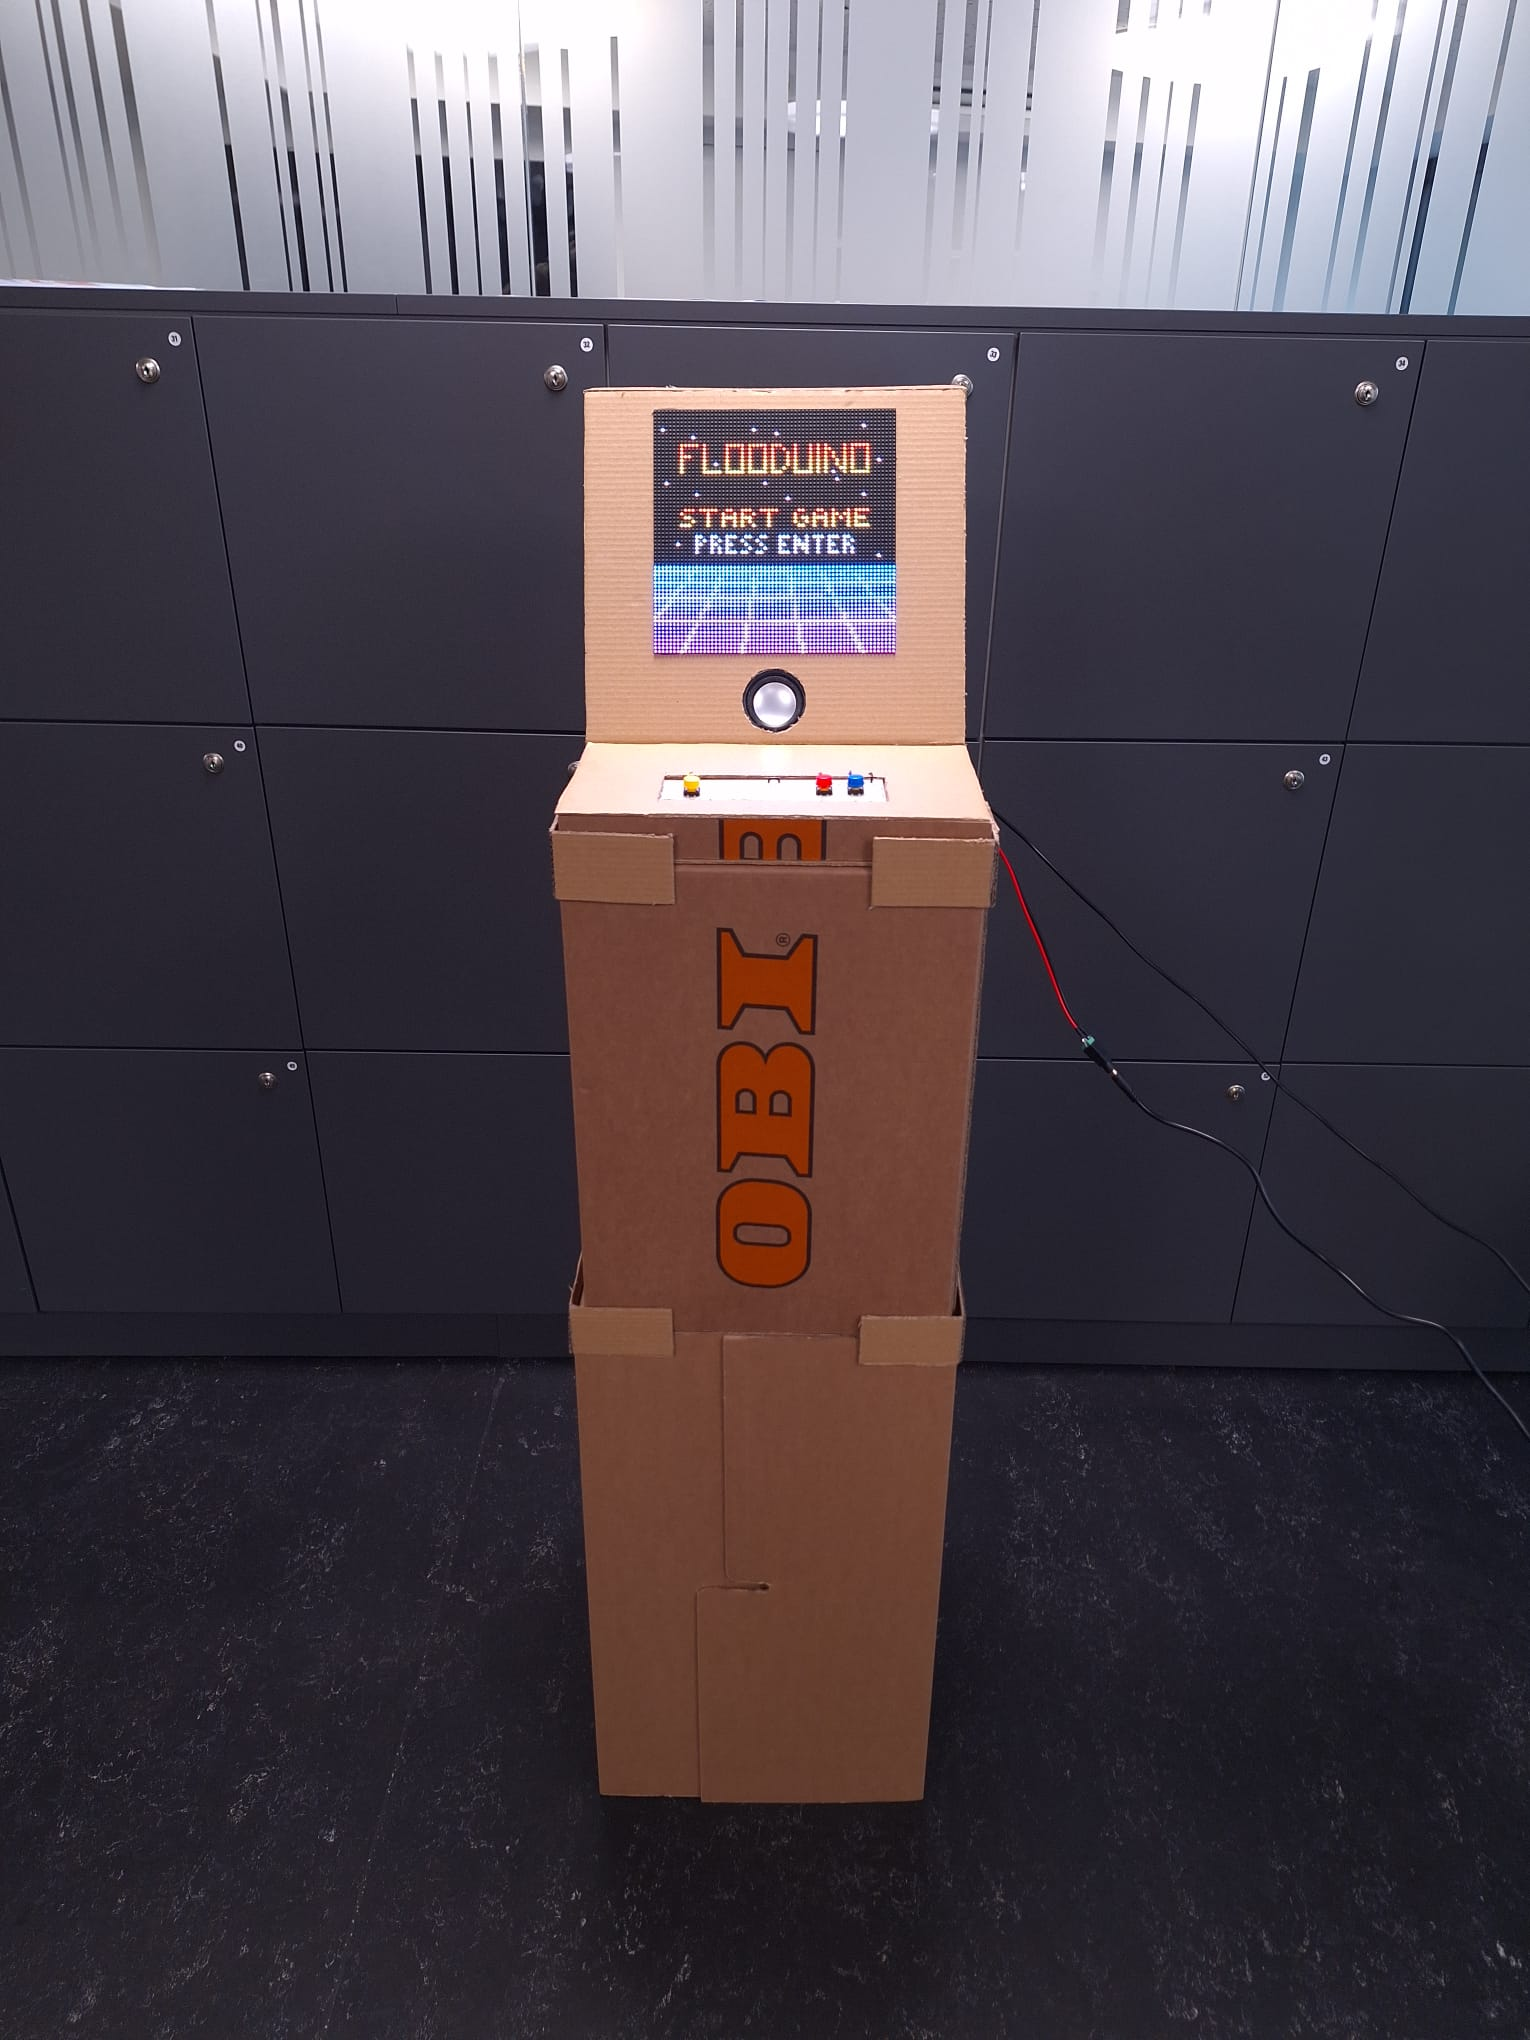
\includegraphics[width=\linewidth]{Finished_Product.jpg}
    \caption{The finished product.}
    \end{minipage}
    \hfill
    \begin{minipage}{0.48\linewidth}
    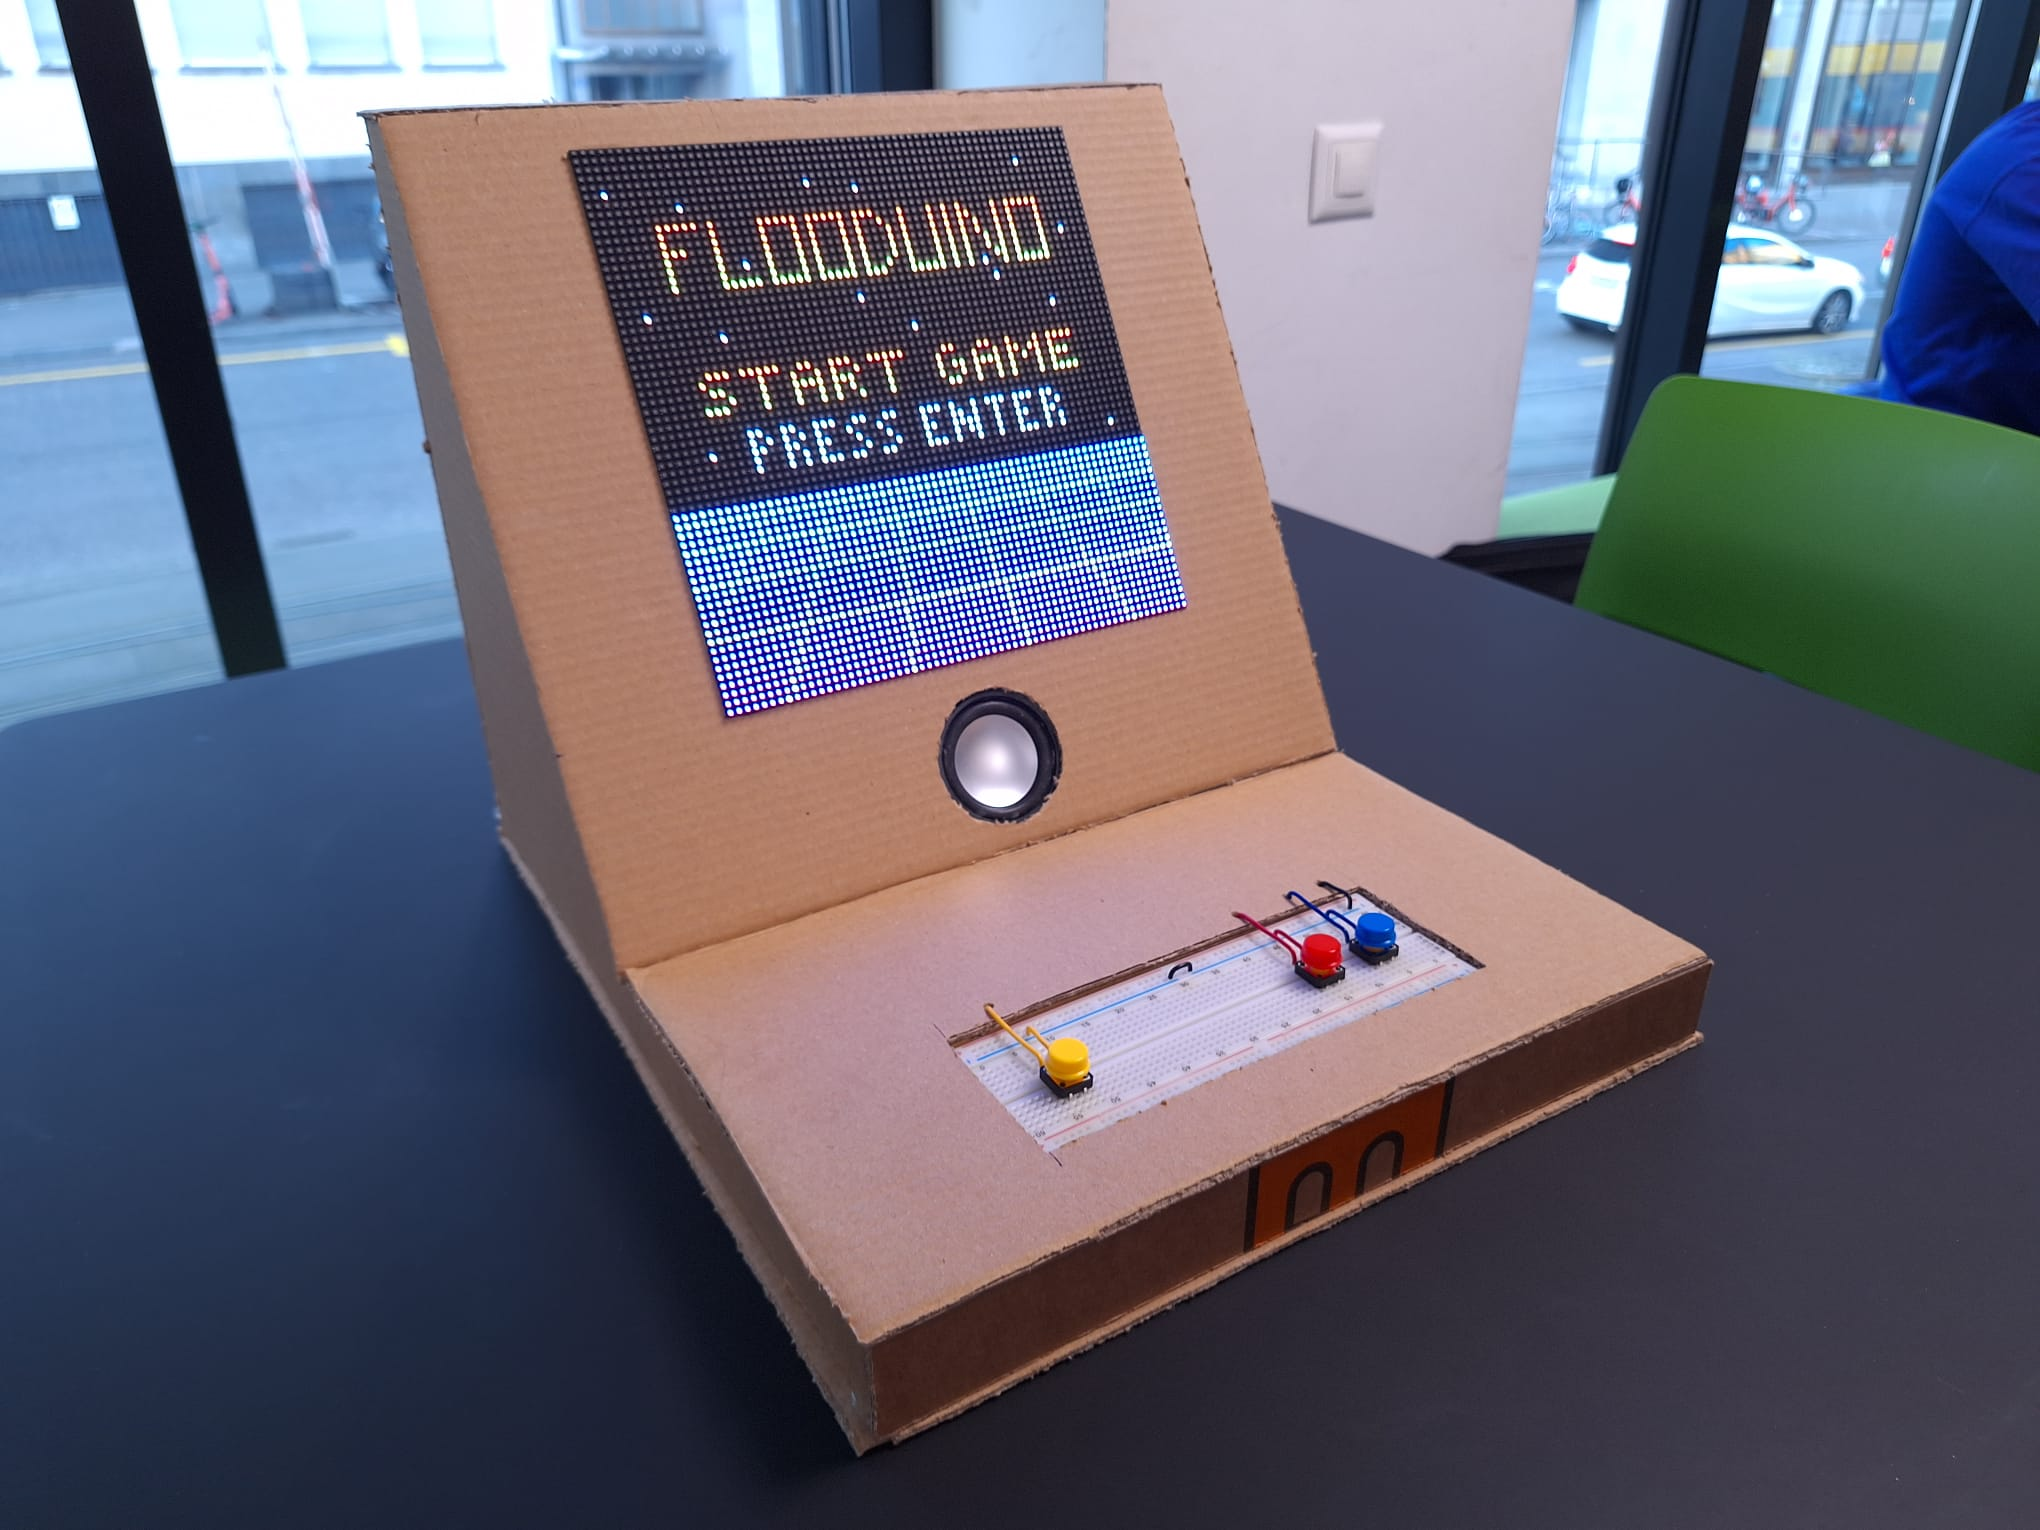
\includegraphics[width=\linewidth]{top_part.jpg}
    \caption{The top part of the housing.}
    \end{minipage}
\end{figure}

\section*{Methodology}

\subsection*{Prototype}

It is necessary to quickly mention the prototype we had created, because it was an important step of our process, as it allowed us to implement the game logic without having connected all the necessary hardware components. It was made completely in C using the raylib graphics library for visual output and ran on our personal computers. We did this to separate the software and hardware problems as much as we could, as we weren't familiar with the hardware components we were to use. We structured our software into the following modules to make porting it to the Arduino easier: input, game logic and output. The input module's function is to detect any button presses made while the game is running. The output module implements some methods which are used to update the window in which the game is shown. To achieve this we used the raylib library. The game logic module is the entry point of the game and uses the aforementioned modules to bring the whole program together. Additionally we used global variables to share the game state between modules.

\begin{figure}[h]
\centering
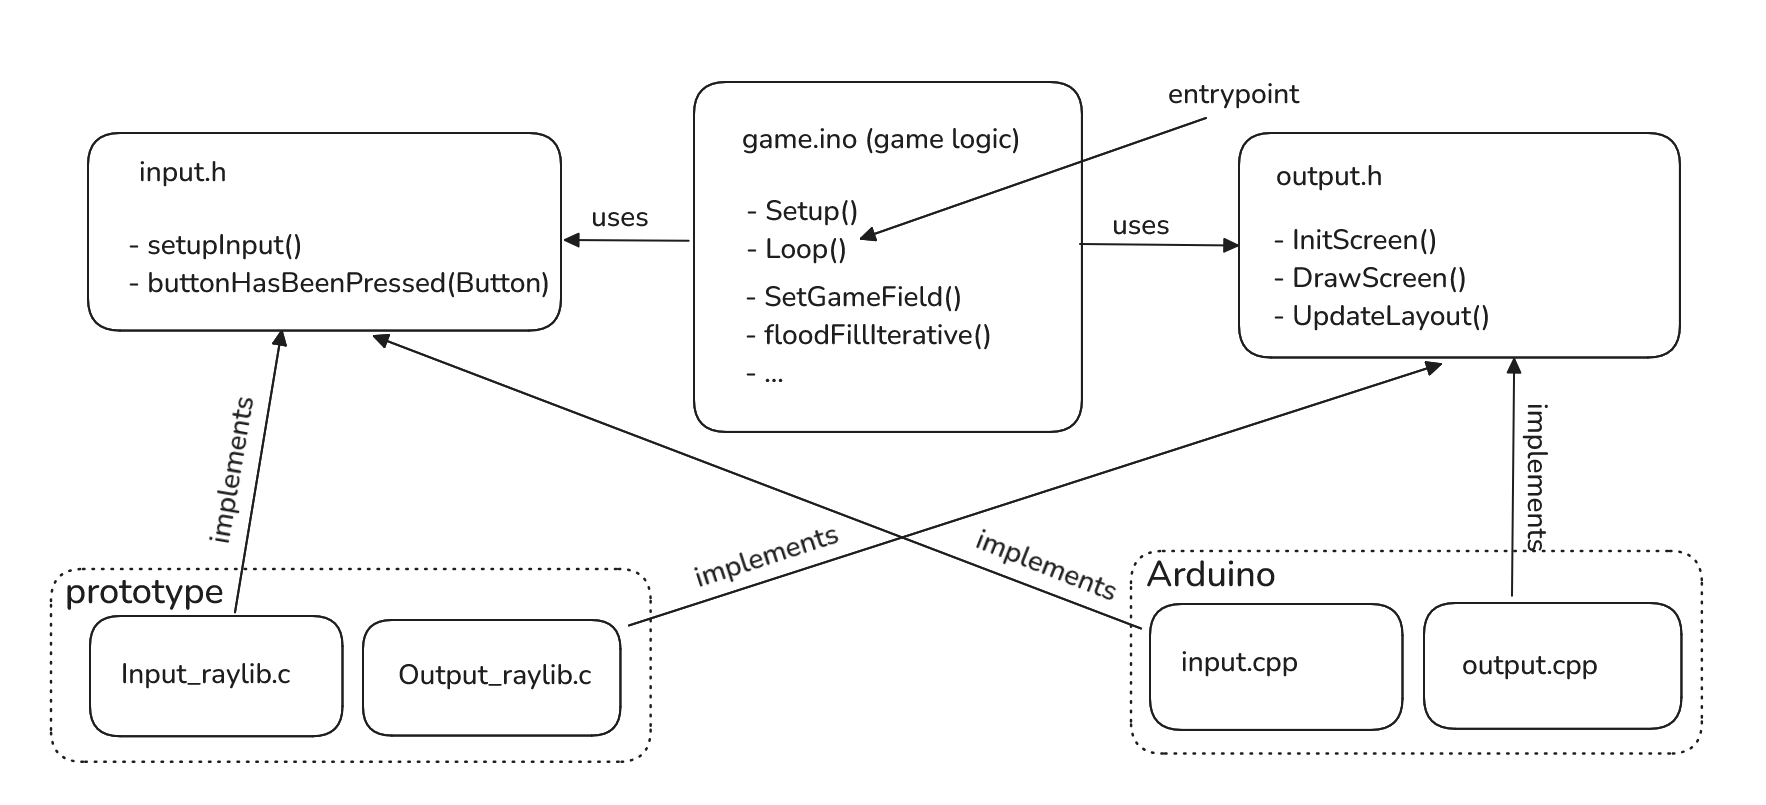
\includegraphics[width=\textwidth]{module_structure.png}
\caption{Structure of the modules for our project.}
\end{figure}
% modulstrucktur einfügen


\subsection*{Porting of the Game to the Hardware}
We were relieved to find out that the porting was relatively straightforward. The main game logic which comprised most of the code needed no further changes and we were able to just copy it over. By using the Adafruit GFX library as output and three buttons on the breadboard as input we were able to quickly confirm that our hardware was working, although it wasn't perfect yet. During this process we also decided to add some music to the game to improve the experience of playing the game, which also came with some challenges, see \nameref{sec:challenges}.

\subsection*{Schematics and Hardware Used}
% bild von schematics/hardware liste einfügen 
\begin{itemize}
    \item DFPlayer mini MP3 Player Module
    \item Speaker 4Ohm 3W 50mm
    \item Buttons for breadboard (3 pcs)
    \item USB b cable
    \item Arduino Mega 2560 Rev3
    \item 9V 1A Power Supply for the Arduino Mega
    \item RGB P3 Matrix Panel 64x64 HUB75
    \item 5V DC 5A Power Supply 5.5mm/2.1mm Plug for the Display
    \item some jumper wires
    \item breadboards (2 pcs)
    \item transistors s9018 h331 (2 pcs)
    \item 1k Ohm resistors (2 pcs)
    \item 10 Ohm resistor
    \item some cardboard boxes and hot glue
\end{itemize}

\subsection*{Input}
The buttons work using interrupts. Every time a button is pressed an interrupt is triggered which increases an internal variable which tracks how often a button has been pressed. This allows us to register any button presses regardless of what the processor is doing. The game loop will check for each counter if it is bigger than zero and perform actions accordingly. Each time the state of such a counter is queried, it is decremented.

\subsection*{Visuals}

\subsection*{Audio}
We decided at the beginning of the assembly of our arcade that we wanted to implement music for the game to enhance the experience for the player. We ended up deciding that every stage of the game has its own song in a loop. This was to be achieved using the DFplayer Mini which operates independently from the Arduino, playing music saved on an inserted sd card. Additionally to this we acquired a speaker for auditory output.

\subsection*{Housing}

The housing was the last thing we decided on and built. Since the game and the hardware used is reminiscent of old arcade games like PAC-MAN we decided to go with a similar look for the housing. To achieve this look we built the entire casing out of cardboard and hot glue. Our approach was to stack two cardboard boxes on top of each other and then put the top piece with the components, screen, speaker and buttons on top of that. The top piece was built by cutting out the individual faces and gluing them together using hot glue.


\section*{Challenges}
\label{sec:challenges}

\subsection*{Displaying Images}
One challenge we faced was to figure out how to display images on the LED-matrix. This was especially difficult since there was no clear guide on how to do this. Our basic idea is to convert the image to an array of rgb values, using a Java program, and store this array on the Arduino which can then be displayed with the Adafruit library. However this process was not straight forward as the colors have to be stored as 16-bit values compared to the normal 32 and each value has to be split and stored in two sequential fields of the array. To add to this there still remains some uncertainty about the exact order every value has to have. This process required a lot of testing and experimenting but in the end we managed to get it to work. 

\subsection*{Audio}
Initially we intended to use a serial connection to control the speaker but this didn't work in combination with the Adafruit GFX library. To circumvent this we communicated with the DFPlayer mini via it's IO1 and IO2 pins to change volume and skip as well as loop songs. Normally this is achieved using button presses but since the music should work independently of the input we used transistors to simulate button presses. Using this the game increases the volume at the start of the game and skips to the next song if the stage is changed. If a song is over we skip ahead until the same song is playing again to loop the song indefinitely. \\\\
After putting all the connected hardware components into the housing, this music control didn't work correctly at times. We suspect that this was caused the wires and transistors that are involved in controlling the DFPlayer Mini being too close to the speaker, which with it's changing magnetic field caused interferences. Placing some cardboard between the speaker and the rest of the hardware fixed this issue. 

\subsection*{Buttons}
A challenge we faced here where the high bounce times of the buttons. A bounce describes the period after a button has been pressed where rapid oscillations trigger multiple unwanted button presses. To deal with this we used a debounce period in which any further button presses are ignored. This was ultimately put at 250 milliseconds which is quite a long time. This leads to the truncation of any button clicks which where made in rapid succession. However, in our experience this is rarely a problem since the game does not require rapid button presses. 

\section*{Division of Labor}
During the project the areas that where worked on by only certain members of the group are listed below:\\\\
Alex: Input, visual design and displaying images.\\
Pascal: Visual output and porting.\\
Frederic and Istref: Game logic and audio.\\\\
Furthermore there where many challenges we worked on together as a team, these include choosing the parts, building the housing, implementing and debugging the speaker, testing and choosing the music.

\section*{Conclusion}

If we could start over again we would be more careful with the usage of libraries and their side effects on such constrained hardware (e.g. Adafruit GFX making the serial connection impossible). 
Additionally we would design the housing for easier access to the hardware and with some more space. We used Git and Github for version control which was very beneficial and we will use it again for future projects. Due to our well structured software we could split the labor evenly. Additionally due to our weekly meetings at Friday on 4:15 pm we were able to make continuous progress and not get too stressed close to the deadline. This was very important since we also learned that each stage took longer than expected. 
Most importantly everyone was motivated and we were able to grow as a group. 


\section*{References}
Inspiration: \url{https://unixpapa.com/floodit/} \\
Libraries used: Adafruit GFX \url{https://github.com/adafruit/Adafruit-GFX-Library} and raylib \url{https://www.raylib.com/} \\
Source of electronics: we ordered from \url{https://www.bastelgarage.ch/} and used some parts that were made available by the University of Basel \\
Code origin (for raylib prototype): \url{https://github.com/raysan5/raylib-game-template}\\
Our repository: \url{https://github.com/AlexMarggraf/Flooduino/}

\end{document}